% Name: Two-to-one multiplexer
% Description: A multiplexer built from a NOT gate, two AND gates, and an OR gate: the select line S passes A to the output when it is 0 and B when it is 1.
% Tags: multiplexer, MUX, logic gates, combinational logic

\usetikzlibrary{circuits.logic.US}

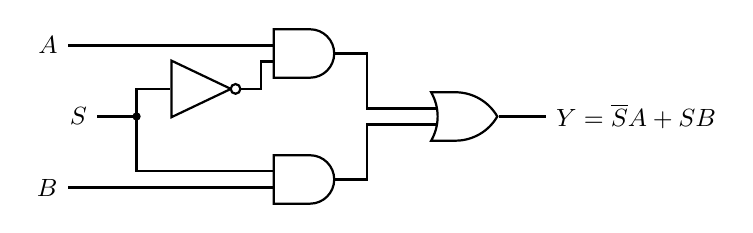
\begin{tikzpicture}[circuit logic US, logic gate input sep=0.17cm, thick, every circuit symbol/.style={thick}, every node/.style={font=\small}]
  \node[and gate] (a1) at (3,1.6) {};
  \node[and gate] (a2) at (3,0) {};
  \node[or gate] (o) at (5,0.8) {};
  \node[not gate] (inv) at (1.6,1.15) {};
  \draw (a1.input 1) -- ++(-2.6,0) node[left] {$A$};
  \draw (a2.input 2) -- ++(-2.6,0) node[left] {$B$};
  % S comes in between A and B and splits: through the inverter to the upper AND, straight to the lower one
  \coordinate (s) at (0.9,0.8);
  \draw (0.4,0.8) node[left] {$S$} -- (s) |- (inv.input);
  \draw (s) |- (a2.input 1);
  \fill (s) circle (1.5pt);
  \draw (inv.output) -- ++(0.25,0) |- (a1.input 2);
  \draw (a1.output) -- ++(0.4,0) |- (o.input 1);
  \draw (a2.output) -- ++(0.4,0) |- (o.input 2);
  \draw (o.output) -- ++(0.6,0) node[right] {$Y = \overline{S}A + SB$};
\end{tikzpicture}
